\documentclass[aspectratio=169,11pt]{beamer}

% ── Theme & Colors ──────────────────────────────────────────────────
\usetheme{metropolis}
\usepackage{appendixnumberbeamer}
\definecolor{strand}{RGB}{31,119,180}   % blue
\definecolor{coil}{RGB}{148,103,189}    % purple
\definecolor{helix}{RGB}{214,39,40}     % red
\definecolor{offset}{RGB}{44,160,44}    % green
\definecolor{outlier}{RGB}{180,180,180} % grey

% ── Packages ────────────────────────────────────────────────────────
\usepackage{graphicx}
\usepackage{booktabs}
\usepackage{multirow}
\usepackage{amsmath}
\usepackage{tikz}
\usetikzlibrary{arrows.meta,positioning}

% ── Footer: slide N/total ───────────────────────────────────────────
\setbeamertemplate{frame numbering}{\insertframenumber/\inserttotalframenumber}

% ── Title ───────────────────────────────────────────────────────────
\title{TriZOD --- Project Update}
\subtitle{LACS Integration, Duplicate Entries \& BindBox Comparison}
\date{22 April 2026}
\author{Tobias Senoner}
\institute{TriZOD Project Meeting}

\begin{document}

\maketitle

% ═══════════════════════════════════════════════════════════════════
% SECTION: LACS Integration Results
% ═══════════════════════════════════════════════════════════════════
\section{LACS Integration Results}

% ── SLIDE: LACS Offset Distribution ────────────────────────────────
\begin{frame}[shrink=5]{LACS Offset Distribution Across the BMRB}

\begin{columns}[T]
\begin{column}{0.55\textwidth}
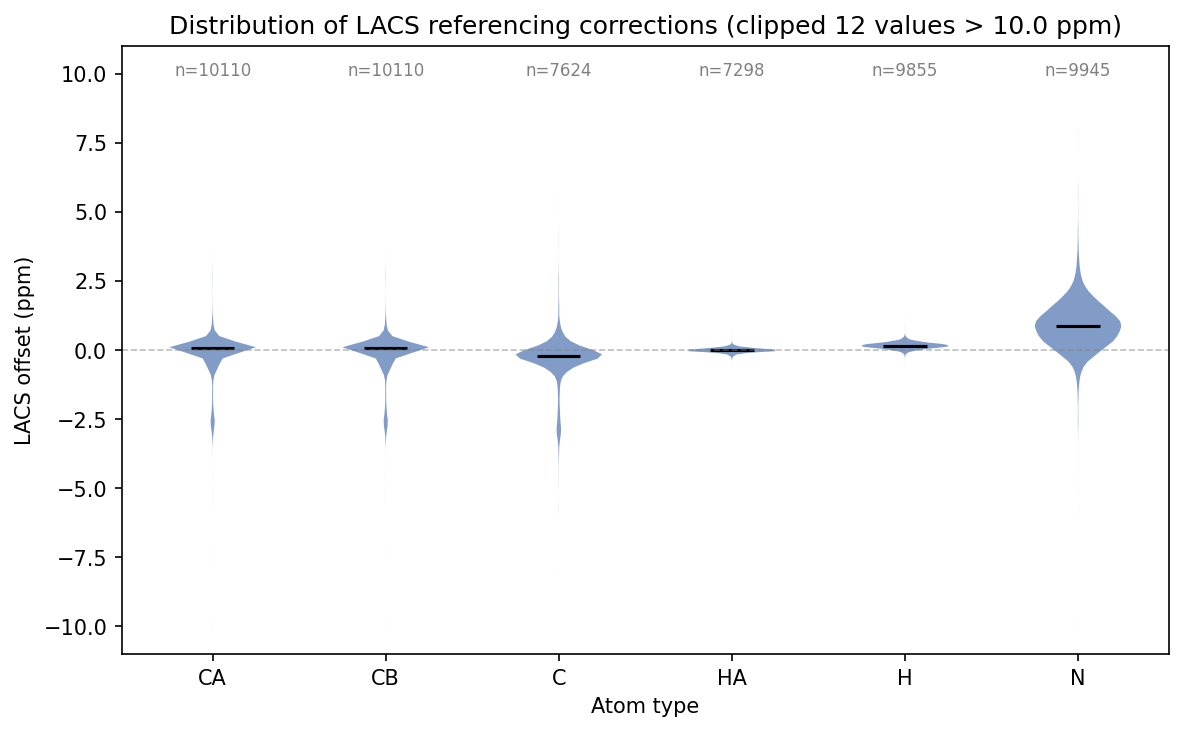
\includegraphics[width=\textwidth]{lacs_offset_violin.png}
\end{column}

\begin{column}{0.42\textwidth}
LACS offsets computed for \textbf{$\sim$10,000 BMRB entries} per atom type.

\medskip
\textbf{Key observations:}
\begin{itemize}\setlength\itemsep{2pt}
  \item CA/CB: tightly centered, $\sim$20\% show $>$0.5~ppm offsets
  \item C$'$: widest ${}^{13}$C spread (up to $\pm$5~ppm)
  \item HA/H: very narrow (${}^{1}$H scale)
  \item \textbf{N: largest offsets}, broad distribution, systematic positive bias ($\sim$35\% mis-referenced)
\end{itemize}

\medskip
\footnotesize
12 entries with offsets $>$10~ppm clipped.
\end{column}
\end{columns}
\end{frame}

% ── SLIDE: LACS Effect on G-scores (by tier) ──────────────────────
\begin{frame}{Effect of LACS Pre-Correction on G-Scores}

\begin{center}
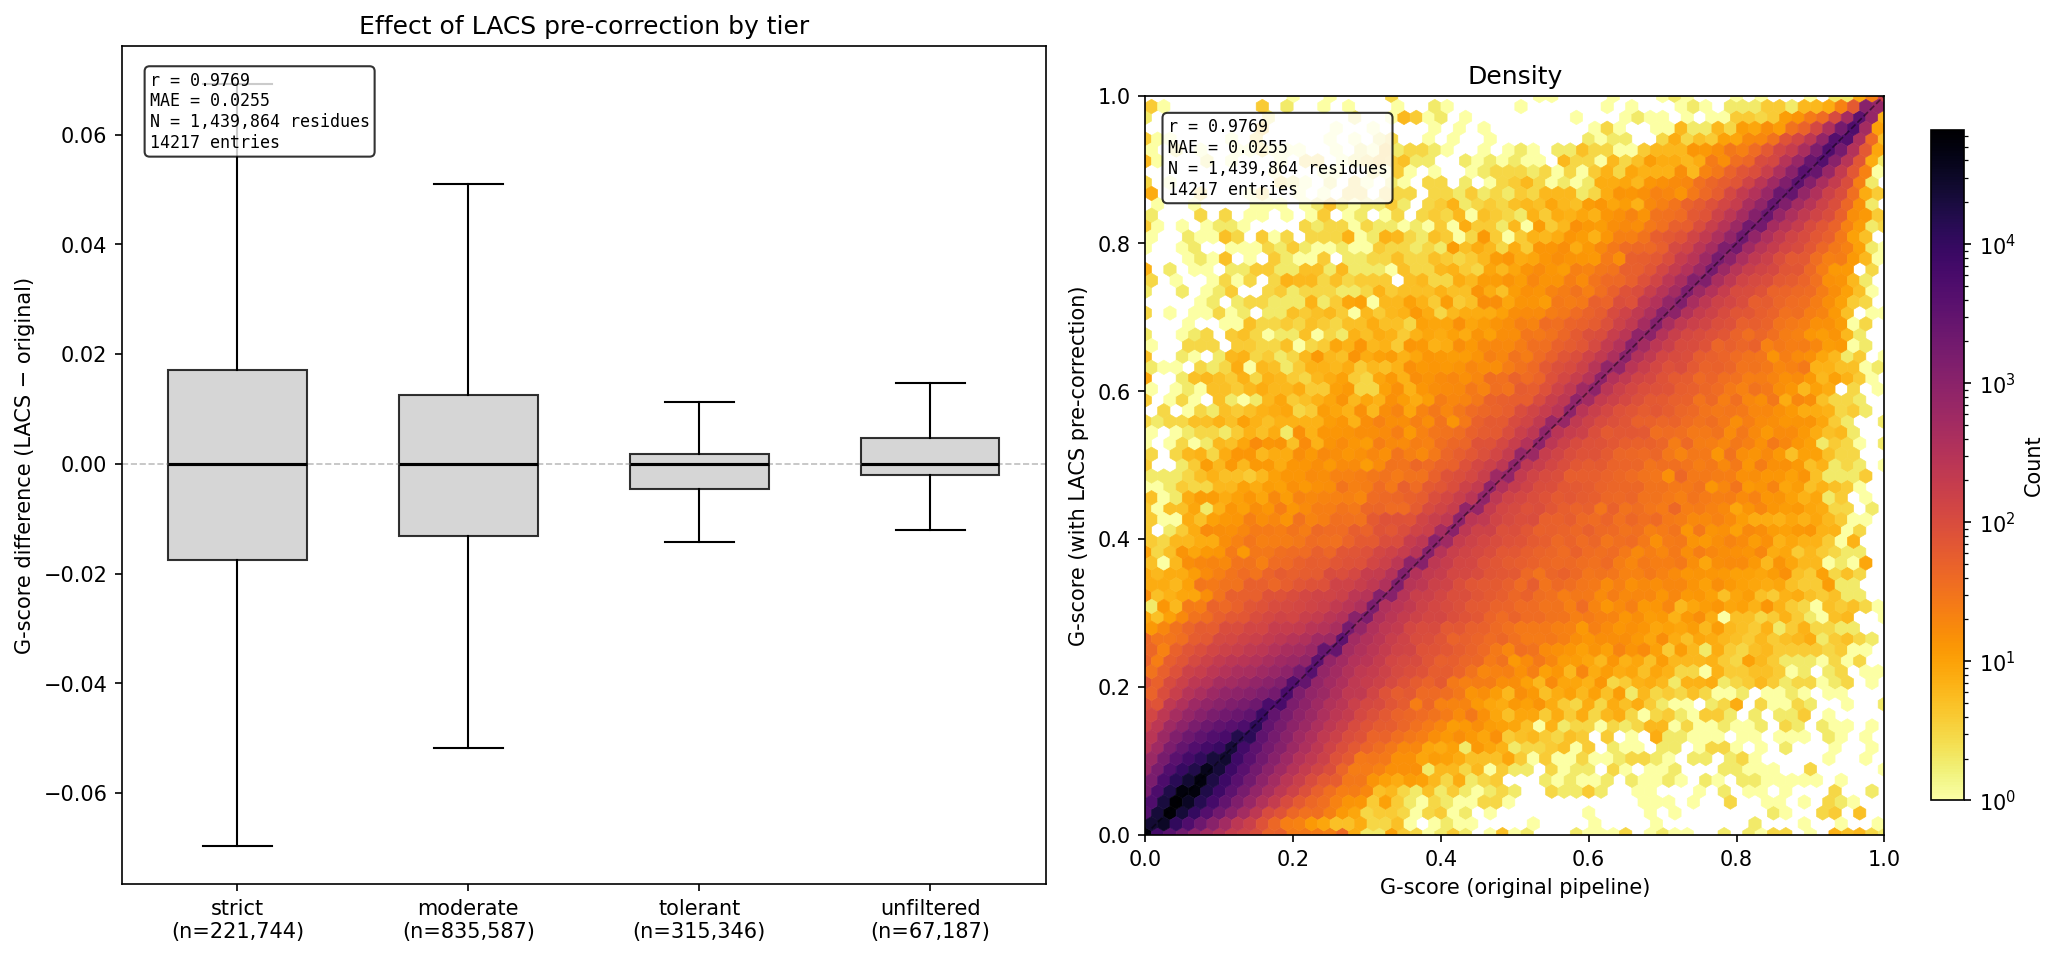
\includegraphics[width=\textwidth]{gscores_lacs_comparison_full.png}
\end{center}

\end{frame}

% ═══════════════════════════════════════════════════════════════════
% SECTION: Duplicate Entry Analysis
% ═══════════════════════════════════════════════════════════════════
\section{Duplicate Entry Analysis}

% ── SLIDE: Duplicate Entries Overview ──────────────────────────────
\begin{frame}[shrink=5]{Same Protein, Multiple Experiments}

\textbf{5,393 entries} across \textbf{1,939 unique sequences} with $\geq$2 BMRB entries.

\medskip
Matching criteria: temperature within 10\,K, pH within 1.0.

\medskip
\begin{center}
\footnotesize
\begin{tabular}{lrrr}
\toprule
\textbf{Protein} & \textbf{Len} & \textbf{Entries} & \textbf{Bound} \\
\midrule
$\alpha$-synuclein             & 140 & 62 &  1 \\
human TSG-6                    &  98 & 33 & 18 \\
Protein-export protein SecB    & 155 & 28 &  0 \\
AbpSH3                         &  59 & 25 &  0 \\
\bottomrule
\end{tabular}
\end{center}

\medskip
\textbf{Two questions:}
\begin{enumerate}
  \item How reproducible are independent measurements of the \emph{same} state?
  \item Can we detect \textbf{binding-induced} shift changes above the noise floor?
\end{enumerate}
\end{frame}

% ── SLIDE: Bound vs Unbound ───────────────────────────────────────
\begin{frame}[shrink=5]{Bound vs.\ Unbound Shift Differences}

\textbf{581 bound/unbound pairs} compared (mean absolute shift difference):

\medskip
\begin{center}
\footnotesize
\begin{tabular}{lccccc}
\toprule
\textbf{Atom} & \textbf{Pairs} & \textbf{Mean abs} & \textbf{Median abs} & \textbf{$>$0.5\,ppm} & \textbf{$>$1.0\,ppm} \\
\midrule
CA  & 398 & 0.481 & 0.330 & 22.5\% & 12.3\% \\
CB  & 384 & 0.532 & 0.349 & 24.5\% & 12.2\% \\
C   & 246 & 0.399 & 0.231 & 19.1\% & 10.2\% \\
HA  & 299 & 0.096 & 0.057 &  3.6\% &  0.8\% \\
H   & 542 & 0.139 & 0.079 &  5.9\% &  1.7\% \\
N   & 492 & 0.763 & 0.453 & 32.8\% & 19.0\% \\
HB  & 295 & 0.088 & 0.048 &  2.7\% &  0.6\% \\
\bottomrule
\end{tabular}
\end{center}

\medskip
\textbf{N shows largest binding effects} (median 0.45~ppm), consistent with backbone sensitivity to ligand binding. ${}^{1}$H atoms show much smaller perturbations.
\end{frame}

% ── SLIDE: Reproducibility & Signal ───────────────────────────────
\begin{frame}[shrink=5]{Measurement Reproducibility \& Binding Signal}

\begin{columns}[T]
\begin{column}{0.52\textwidth}
\textbf{Independent measurements} (1,301 pairs):
\footnotesize

\medskip
\begin{tabular}{lcc}
\toprule
\textbf{Atom} & \textbf{Mean abs} & \textbf{Median abs} \\
\midrule
CA  & 0.298 & 0.206 \\
CB  & 0.305 & 0.205 \\
C   & 0.547 & 0.472 \\
HA  & 0.045 & 0.030 \\
H   & 0.069 & 0.049 \\
N   & 0.356 & 0.229 \\
HB  & 0.101 & 0.056 \\
\bottomrule
\end{tabular}

\smallskip
\normalsize
\textit{This is the noise floor} --- variation between independent measurements of the same protein in the same state.
\end{column}

\begin{column}{0.45\textwidth}
\textbf{Binding signal / noise ratio:}
\footnotesize

\medskip
\begin{tabular}{lccc}
\toprule
\textbf{Atom} & \textbf{Binding} & \textbf{Noise} & \textbf{Ratio} \\
\midrule
CA & 0.481 & 0.298 & \textbf{1.6$\times$} \\
CB & 0.532 & 0.305 & \textbf{1.7$\times$} \\
C  & 0.399 & 0.547 & 0.7$\times$ \\
HA & 0.096 & 0.045 & \textbf{2.2$\times$} \\
H  & 0.139 & 0.069 & \textbf{2.0$\times$} \\
N  & 0.763 & 0.356 & \textbf{2.1$\times$} \\
HB & 0.088 & 0.101 & 0.9$\times$ \\
\bottomrule
\end{tabular}

\smallskip
\normalsize
Ratio $>1$: binding effect exceeds noise.

\alert{C and HB are below noise} --- not reliable binding indicators at this scale.
\end{column}
\end{columns}
\end{frame}

% ═══════════════════════════════════════════════════════════════════
% SECTION: BindBox Comparison
% ═══════════════════════════════════════════════════════════════════
\section{BindBox Comparison}

% ── SLIDE: What is BindBox? ───────────────────────────────────────
\begin{frame}[shrink=10]{BindBox: Interactive NMR Shift Analysis}

\textbf{BindBox} (Bind Research, UK) --- Streamlit web app for IDP chemical shift analysis.

\medskip
\textbf{Main tools:}
\begin{enumerate}\setlength\itemsep{2pt}
  \item \textbf{BMRB Dashboard} --- 1D/2D/3D shift distributions, Gaussian fitting, POTENCI overlay
  \item \textbf{SpinForecast} --- Bayesian peak assignment without sequential connectivities
  \item \textbf{POTENCI} --- same algorithm as TriZOD (Nielsen \& Mulder 2018)
  \item \textbf{pH/T Adjustment} --- shift prediction under changed conditions
\end{enumerate}

\medskip
\textbf{Their dataset:}
\begin{itemize}
  \item 3,320 BMRB entries (disordered regions, AlphaFold2 pLDDT $< 70$)
  \item 480,599 shift rows, pre-computed Parquet files
  \item BMRB September 2025 release
\end{itemize}

\medskip
\footnotesize
Preprint in preparation ($\sim$May 2026): probabilistic IDP peak assignment.
\end{frame}

% ── SLIDE: BindBox vs TriZOD ─────────────────────────────────────
\begin{frame}[shrink=5]{BindBox vs.\ TriZOD}

\begin{center}
\footnotesize
\begin{tabular}{lll}
\toprule
\textbf{Aspect} & \textbf{BindBox} & \textbf{TriZOD} \\
\midrule
Interface    & Web GUI (Streamlit)       & CLI + Python library \\
Mode         & Interactive, single-protein & Batch, database-scale \\
Scale        & 3,320 entries             & 17,388 entries \\
Primary output & Visualizations, probabilities & Per-residue Z/G-scores \\
Data storage & Pre-aggregated Parquet    & Raw NMR-STAR + caches \\
Filtering    & User-driven UI controls   & Systematic 4-tier (16 criteria) \\
Referencing  & User-supplied offsets     & LACS automatic detection \\
Peak assignment & SpinForecast (Bayesian) & Not in scope \\
Disorder scoring & Not in scope          & Core purpose \\
Disorder def.  & AlphaFold2 pLDDT        & CheZOD Z/G-score \\
\bottomrule
\end{tabular}
\end{center}

\medskip
\textbf{Complementary, not competitive:} BindBox provides interactive single-protein exploration; TriZOD provides systematic database-scale scoring.
\end{frame}

\end{document}
